\section{Stream-based applications}
\vspace{-10pt}
Traditionally, stream processing has been used in application domains with low tolerance
of failure. Such applications can only produce meaningful results when the processing is carried
out without any loss of data or approximation.
Financial algorithmic trading~\cite{streambase-algo} is a prime example. 
Investment banks, trading on the stock market, need to process a large volume of financial events in
real-time.
Complex algorithms are used to capture the current market situation and to give hints on
profitable trades, exploiting temporary arbitrage conditions. For these applications, the focus is on
efficiency: being able to make a trade even a split second before a competitor is the key to make
profit.
In this scope, the necessity of processing all the available data is evident because a wrong choice
based on approximate data could lead to financial loss.

On the other hand, there are some classes of applications that are able to operate correctly even when
not all the data can be processed. In many cases, a certain degree of failure in the system is
tolerable and does not prevent the application from producing meaningful results.

We will describe two broad classes of applications that can use an approximate result approach.  
The first class are \emph{global sensing infrastructures}~\cite{senseweb,gsn,irisnet}, which are
concerned mostly with sensor data, developing a worldwide infrastructure in which different classes of
sensors can be connected and accessed through a common interface. They allow users to process data
streams generated by different sensor networks.
 
A second class that can benefit from this approach are applications for \emph{real-time
processing of social media events}. These applications analyse the constant stream of user generated
content, extracting useful information from it. It is possible to process user-generated data
streams, for example from Twitter, to understand how the public reacts to a certain product launch or
event~\cite{twitter-sentiment,twitrratr}, identifying trends as they
arise~\cite{twitter-stocks,twitter-sentiment-1}. It also possible to exploit the locality
information disclosed by the users in order to identify differences in lifestyle and
preferences, as done by FourSquare~\cite{foursquare-wsj,foursquare-rude}.
\vspace{-15pt}
%--------------------------------------------------------------------------------------------------------
\subsection*{Environmental Monitoring}
\label{envmon}
%\vspace{-10pt}
The first domain of applications that we will take into consideration are related to large-scale
scientific sensing, in particular we will describe projects dealing with large-scale environmental
monitoring.  In recent years, the availability of cheap micro-sensing technology has unleashed sensing
at an unprecedented scale. We can expect in the future to see everything of material significance being \emph{sensor-tagged} and report its state or location in
real-time~\cite{irisnet,qpsn,stream-processing-challanges}. At the present time, a great number of
large-scale sensing projects are being developed and we can expect even more to come soon into
place~\cite{earthscope,neon,casa-lead,swissexp}.

One area in which large-scale sensing has flourished is \emph{environmental monitoring}. The growing
concern about climate change has brought a lot of attention to environmental studies. Many
large-scale sensing projects have been launched to understand better the behaviour of many natural
processes.
Examples of such efforts are, for instance, the Earthscope~\cite{earthscope} and the Neon~\cite{neon}
projects.

Earthscope is a multi-disciplinary project across earth sciences to study the geophysical structure and
evolution of the American continent. It uses a large number of sensors geographically distributed over
the whole continent to answer some of the outstanding questions in Earth Sciences by looking deeper, at
an increased resolution, and integrating diverse measurements and observations.~Thousands of geophysical
instruments measure the motion of the Earth's surface, record seismic waves and recover rock samples from
depths at which earthquakes originate. All the collected data is freely available, and a large community
of scientists is conducting several multidisciplinary studies based on it. Examples of sensing
projects within Earthscope include the constant monitoring of the San Andreas fault and the Plate Bound
Observatory, which collects information about the tectonic movements across active boundary zones.
NEON stands for National Ecological Observation Network. This project aims at creating a new national
observatory network to collect ecological and climatic observations across the United States. It is an
example of a continental-scale research platform for discovering and understanding the impact of climate
change, land-use change and invasive species on ecology. It is the first observatory designed to detect
and enable forecasting of ecological change at continental scales over multiple decades. Obtaining this
kind of data over a \mbox{long time} period is crucial to improving ecological forecast models and will
greatly help understand the effects of human interference on climate. These are just
two examples of large-scale monitoring projects, and many others already exists or will be started in the
near future~\cite{testban,skysurvey,neon,usvo}.

Environmental sensing is a natural application for stream processing systems because a continuous flow of
measurements are generated by a large number of sensors. Stream processing offers an intuitive and
flexible paradigm to harness such a high volume of data. It also gives the possibility of obtaining a
real-time picture of the measured phenomena, enabling quick reaction to possibly disruptive events. The
core components of these projects are sensing stations, which are geographically distributed and
frequently subject to harsh conditions. In such scenarios, the failure of sensing devices is common and
often their replacement is problematic. Long running continuous queries need to be able to handle some missing
data, adapting to the new conditions and reporting the achieved quality of processing. To collect and
process all data at all times remains infeasible, and it is important for the computing backbone of such
projects to be able to withstand a certain degree of failure within the system~\cite{dependable-is-sensing}.
% 
% I will now present a more specific example of infrastructures aiming at supporting large-scale sensing
% projects.  The first is concerned with meso-scale weather monitoring, while the second focuses on the
% collection of data from environmental sensors in a more general purpose fashion. Both project could take
% advantage from my research, by enabling them to produce results in real-time and to better operate in the
% occurrence of failure due to an excessive amount of input data.
\paragraph{Distributed Collaborative Adaptive Sensing.} Meso-scale weather events, such as tornadoes and
hurricanes, cause a large number of deaths and a great deal of damage to infrastructures every year.
Being able to understand and predict when these hazardous weather conditions will occur can greatly
mitigate their consequences.

In this regard, the National Science Foundation has recently established the center for
\textit{Collaborative Adaptive Sensing of the Atmosphere (CASA)}~\cite{casa}. Its goal is to
enhance the current infrastructure of long-range weather observing radars with a large number of small
solid-state radars in order to increase the sampling resolution throughout the entire
troposphere.
Although current \mbox{long-range} radar technology allows the coverage of large areas with a relatively
small number of devices, these are not able to measure correctly the lowest part of the atmosphere in
areas far away from the radar. This is due to the Earth's curvature and terrain-induced blockage.  This
new sensing paradigm, based on a large number of smaller devices, is referred to as \emph{Distributed
Collaborative Adaptive Sensing~(DCAS)}. Distributed refers to the use of numerous small and inexpensive
radars, spread densely enough to measure the area fully, even at lower altitudes at which the traditional
approach fails.
Collaborative refers to the coordination of multiple devices that cover overlapping areas to increase
the resolution and the precision of the measurements compared to a single radar. Adaptive refers to the
ability of the infrastructure to dynamically adjust its configuration based on the current weather
conditions and user needs.
Similar to CASA is the \emph{Linked Environments for Atmospheric
Discovery~(LEAD)}~\cite{lead}. It gives scientists the tools with which they can automatically spawn
weather forecast models in response to real-time weather events in a desired region of interest. It is a
middleware that facilitates the adaptive utilization of distributed resources, sensors and workflows.
While CASA is primarily concerned with the reliable collection of the data, LEAD is the backbone
processing infrastructure. It allows the automation of time consuming and complicated tasks associated
with meteorological science through the creation of workflows. The workflow tool links data management,
assimilation, forecasting and verification applications into a single system. Weather information is
available to users in real-time, not being restricted to pre-generated data, which greatly expands
analysis capabilities.

The integration of these two systems offers a useful infrastructure to atmospheric
scientists~\cite{casa-lead}.  First of all, it allows meteorologists to interact directly with data from
the instruments as well as control the instruments themselves. Unlike traditional forecasting
approaches, it allows the establishment of interactive closed loops between the forecast analysis and the
instruments. This sensing paradigm, based on numerous input devices and the possibility of directly
feeding their data into a forecasting model, is changing the way meso-scale weather events are detected
and will help mitigate their impact. Stream processing has the potential of enhancing the CASA/LEAD
infrastructure, extending its real-time monitoring capabilities.
% In this infrastructure, when implemented
% at larger scale, failure is going to be the common case. CASA is built from small weather stations, and
% it is designed to withstand failure at the sources and to reconfigure at run-time~\cite{casa}. This means
% that during long running queries, the backbone processing system is likely to be affected by failure at
% the sources and experience variations in the quality of the results.  For these reasons, this scenario
% would be a prefect test-bed onto which exploring ways to operate a large-scale monitoring system under
% constant partial failure, while constantly measuring the achieved quality-of-service.

% \paragraph{The Swiss Experiment} Another example of large-scale environmental sensing project is
% represented by the Swiss Experiment~\cite{swissexp}. The aim of the project is to enable effective
% real-time environmental monitoring through wireless sensor networks and a modern, generic
% cyber-infrastructure. It is a collaborative projects with many contributions on different scientific
% and technological aspects.
%  Within the scope of the project, a new wireless sensor network technology has been developed, called
% SensorScope~\cite{sensorscope}. This is an out-of-the-box environmental monitoring infrastructure based
% on inexpensive wireless sensor nodes. SensorScope is both a hardware and software architecture. It
% falls into the category of time-driven networks, as the stations intermittently transmit environmental
% data to a sink, which in turn make the received data available through a number of interfaces. It has
% been deployed and tested in many occasions, being one of the fundamental building block employed in the
% project. It was used to monitor the quality of the water in the Le Boiron de Morges river, on Le Genepi
% rock glacier, to monitor dangerous mud streams, and on the Grand St.  Bernard pass, to obtain a very
% precise map of evaporation of the area.
%  PermaSense~\cite{permasense} is another technological effort within the project. It aims at the
% development of an innovative sensor infrastructure for automated, unattended long-term data acquisition
% in the extremes of high-alpine regions. The goal is to investigates the effect of permafrost in
% high-alpine environments.
%  All the data gathered by the project is made available through a number of interfaces like GoogleMaps
% and SenseMap~\cite{sensemap}. The acquisition and storage of the data is also performed in different
% ways. It is saved in a wiki, in comma separated values files, even though the most interesting way is
% through the GSN (Global Sensor Networks).  This is a database software middleware designed to
% facilitate the deployment and programming of sensor networks. Large-scale, long-running monitoring
% tasks like the ones in the aims of the Swiss Experiment are likely to experience failure, either at the
% sources and in the distributed backbone processing infrastructure. GSN, the tool employed for
% \mbox{real-time} data mining within this project, reacts to failure by simply releasing the associated
% resources and continuing the processing without them~\cite{gsn-book}. This behaviour could be improved,
% by introducing the ability of introducing quality-awareness in its processing. Extending GSN in this
% regard, would allow it to better operate in hostile environments characterized by a high occurrence of
% failure. This would enhance its capabilities, providing users with a better understanding of
% approximate results and the behaviour of the system.


% \begin{figure}[b!] \centering 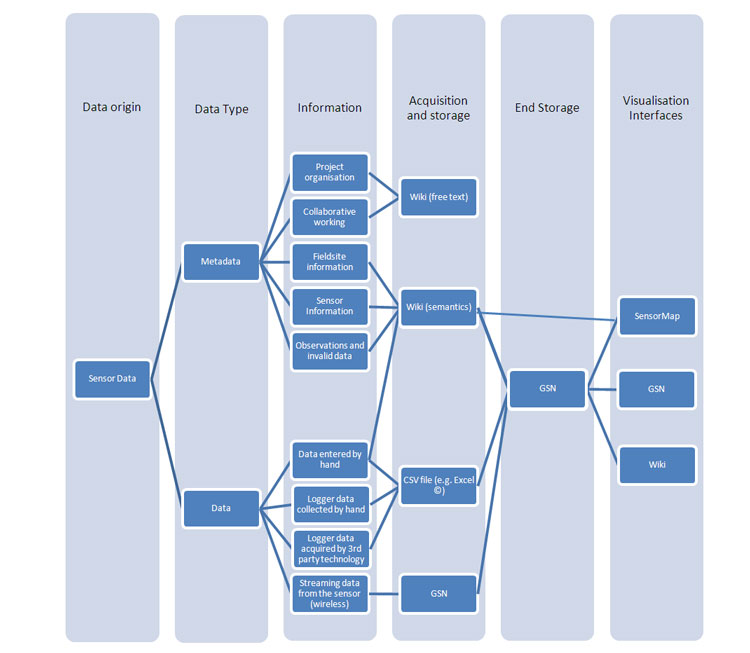
\includegraphics[scale=0.4]{img/swissex-overview.jpg} \label{img:swissex}
% \caption{Outline of the SwissEx infrastructure} \end{figure}


% \subsubsection*{Astrophysics} 
\label{sec:astro} 
%\notemf{I find the structure here to be a little confusing. Some options: a) eliminate astrophysics b) talk of swiss
%experiment in the introduction of the paragraph, as it is a more general purpose experiment c) leave it like this d)
%your say?}

\begin{structure}
	\item Application of StreamGlobe, explained in Section \ref{sec:streamglobe}
\end{structure}

StarGlobe: Grid-Based Data Stream Processing in e-Science \cite{starglobe-grid}

%--------------------------------------------------------------------------------------------------------
\subsection*{Real-time Social Media Analysis}

Social networks have experienced a large growth over the past years~\cite{flickr-growth}, changing the
Internet landscape by shifting the balance of the available information towards user-generated content.
Numerous sites allow users to interact and share content based on social links. Users of these networks
often establish hundreds or even thousands of social links with other users, constantly reshaping the
social graph~\cite{fb-interactions}.
Users share photos~\cite{flickr, facebook}, videos~\cite{youtube}, status updates~\cite{twitter} and
locations~\cite{foursquare}, providing a continuous stream of valuable information for researchers and
companies. 
Social media analysis has become an essential tool for online marketing, and many tools have been
developed to help discovery and to reach new potential customers~\cite{wildfire, brandwatch}. The
possibility to target specific segments of the online population with customised advertisements allows
companies to increase their return on investment and users to avoid unwanted communication.
Furthermore, by analysing Twitter streams, it is possible to predict in real-time the evolution of
numerous phenomena, such as the spreading of diseases~\cite{mappyhealth} or the fluctuation of stock
quotes~\cite{twitter-stocks}. Other applications analyse keywords in status updates to determine the
public sentiment towards a certain topic, brand or public figure~\cite{socialmention, twendz, tweetfeel}.
The diffusion of user-generated content through a social network is referred to as a \emph{social
cascade}. The next section describes social cascades and explains why their prediction can be useful for
the correct allocation of resources in content distribution networks.
% 
% \section{Twitter Analisys Tools}
% 
% Many tools have been developed to extract information from Twitter statuses. Th
% 
% 
% \emph{Social Mention}~\cite{socialmention} is a tool that allow the tracking of certain keywords across
% over 80 social networks. It monitors the status update streams produced by users of the major social
% networks and it filters only those containing a certain keyword. It provides a list of all statuses
% together with a number of statistics. It is possible for instance to monitor how many people mention the
% keyword, what sentiment are expressed in the statuses, what other keywords appear the most together with
% the status. One of the aims of this tools is to help marketers to assess the perception of a brand or to
% measure the impact of media campaign. 
% \emph{Strength} is the likelihood that a certain brand is being discussed on social media, given by
% phrase mentions within the last 24 hours divided by total possible mentions. \emph{Sentiment} is the
% ratio of mentions that are generally positive to those that are generally negative. \emph{Passion} is a
% measure of the likelihood that individuals talking about a brand will do so repeatedly. \emph{Reach} is 
% a measure of the range of influence. It is the number of unique authors referencing a brand divided by
% the total number of mentions. 
% 
% 
% 
% 			\bul{Overview of trends in social networks}
% 			% \incite{social-networks}
% 
% 			\incite{storm} 
% 
% 			\bul{Twitter Analysis Tools}
% 			%\incite{socialmention}
% 			\incite{twitrratr}
% 			\incite{twitter-sentiment}
% 			\incite{ubervu}
% 			\incite{twendz}
% 			\incite{tweetfeel}
% 
% 			\bul{FourSquare Articles}
% 			\incite{foursquare-wsj}
% 			\incite{foursquare-rude}	
% 
% 			\bul{Papers on Twitter sentiment analysis}
% 			\incite{twitter-stocks}
% 			\incite{twitter-sentiment-1}
% 			\incite{twitter-sentiment-2}
% 			\incite{twitter-sentiment-3}
% 			\incite{twitter-sentiment-4}
% 			\incite{twitter-sentiment-5}
% 
% 			\bul{Papers on Social Casacades}
% 			\incite{buzztraq}
% 			\incite{socialcascade-flickr}
% 			\incite{socialcascade-salvo}
% 
% 
% % social cascades
\paragraph{Social Cascades.} One interesting application of social media real-time analysis is the
possibility of predicting social cascades. A \emph{social cascade} is the phenomenon generated by the
repeated sharing of a certain content over an Online Social Network (OSN). One person discovers an
interesting piece of information and shares a link to it with a few friends, who share it themselves and
so on. When content is considered interesting by a community, it starts being shared over and over again,
possibly reaching a large number of hits in a short period of time~\cite{socialcascade-flickr}. Due to the
characteristics of social networks, this process mimics the spread of an epidemic~\cite{buzztraq}.
Initial studies about this phenomenon date back to the 1950s, with the theory
of Diffusion of Innovation~\cite{diffusion-innovation}. It is only now though, with the wealth of
information shared through OSNs, that is possible to study social cascading in much more detail.

More formally, a user \emph{Bob} is reached by a social cascade when he receives a certain content
\emph{c} and:
\begin{enumerate}
\singlespacing
	\item User \emph{Alice} already posted content \emph{c} before user \emph{Bob}; and
	\item There is a social connection between users \emph{Alice} and {Bob}.
\end{enumerate}
\paragraph{Social Cascading in Twitter.}
The diffusion of links through Twitter can be used to understand better what a social cascading tree
looks like. Twitter is a micro-blogging website on which users can share a short message of maximum 140
characters with other users called ``followers''. In this particular social network, it is also possible
to characterise cascades further into two main groups: L-cascades and RT-cascades~\cite{outweeting}.

L-cascades occur when a certain content is shared by direct followers. More formally, we can
say that an L-cascade is the graph of all users who tweeted about a certain content \emph{c}. A cascade
link is formed when (1) Users \emph{Alice} and \emph{Bob} shared content \emph{c}, (2) User
\emph{Alice} posted \emph{c} before user \emph{Bob}, and (3) User \emph{Bob} is a follower of user
\emph{Alice}.

Instead, RT-cascades do not only take into account direct connections but also the
possibility of crediting certain content to a user even without being a direct follower. If user
\emph{Bob} wants to give credit to user \emph{Alice} for certain content, he prepends his new tweet
with the conventional \emph{RT @Alice} tag followed by the original tweet. In this way, \emph{Bob} gives
direct credit to \emph{Alice} for the content of the tweet even without being a direct follower. This
phenomenon is known as ``retweetting''~\cite{retweet}. More formally, we can say that an RT-cascade
\emph{R(c)} is the graph all the users who have retweeted content~\emph{c} or have received credit for
it.
A cascade link is formed when (1) User \emph{Bob} tweeted about content \emph{c}, (2) User \emph{Alice}
tweeted about content \emph{c} before user \emph{Bob}, and (3) User \emph{Bob} credited user \emph{Alice}
as the original source of the content.
\vspace{-0.5cm}
\paragraph{Impact of Social Cascades on CDNs.}
% CDN
It is difficult to predict where and when certain content will become popular.
Many content providers rely on Content Delivery Networks (CDNs) to distribute their content across
multiple geographic locations in order to enhance the availability of their content to their users. The
choice of \emph{what} content to replicate, \emph{where} and for \emph{how long} is crucial to the
reduction of the costs associated with the use of a CDN. Being able to predict the popularity of certain
content is needed for the correct provisioning of resources. For example, it has
been found that the top 10\% of the videos in a video-on-demand system account for approximately 60\% of
accesses, while the rest of the videos (\ie the 90\% are the tail) account for
40\%~\cite{buzztraq}.

An attempt to characterise the spread of social cascades focuses on improving the caching of
content, exploiting the geographic information from the cascades~\cite{socialcascades-salvo}.
This approach leverages the observation that a social cascade tends to propagate in a geographically
limited area, because social connections typically reflect real life relationships. It is
also likely that a video spoken in a particular language would tend to propagate within the national
borders of a country, in which that language is native. Based on an analysis of a corpus of 334 millions messages
shared on Twitter, extracting about 3 millions single messages with a video links, it was found that
about 40\% of hops in social cascades involve users that are, on average, less than 1,000 km away from
each other.

% 